\documentclass[11pt]{article}

\usepackage{epsfig}
\usepackage{amsfonts}
\usepackage{amssymb}
\usepackage{amstext}
\usepackage{amsmath}
\usepackage{xspace}
\usepackage{theorem}
\usepackage{graphicx}
\usepackage{tikz}
\usepackage{pgfplots}

% \usepackage{layout}% if you want to see the layout parameters
% and now use \layout command in the body

% This is the stuff for normal spacing
\makeatletter
 \setlength{\textwidth}{6in}
 \setlength{\oddsidemargin}{0in}
 \setlength{\evensidemargin}{0.5in}
 \setlength{\topmargin}{0in}
 \setlength{\textheight}{9in}
 \setlength{\headheight}{0pt}
 \setlength{\headsep}{0pt}
 \setlength{\marginparwidth}{59pt}

 \setlength{\parindent}{0pt}
 \setlength{\parskip}{5pt plus 1pt}
 \setlength{\theorempreskipamount}{5pt plus 1pt}
 \setlength{\theorempostskipamount}{0pt}
 \setlength{\abovedisplayskip}{8pt plus 3pt minus 6pt}


\newenvironment{proof}{{\bf Proof:  }}{\hfill\rule{2mm}{2mm}}
\newenvironment{proofof}[1]{{\bf Proof of #1:  }}{\hfill\rule{2mm}{2mm}}
\newenvironment{proofofnobox}[1]{{\bf#1:  }}{}
\newenvironment{example}{{\bf Example:  }}{\hfill\rule{2mm}{2mm}}


\newtheorem{theorem}{Theorem}
\newtheorem{lemma}[theorem]{Lemma}
\newtheorem{proposition}[theorem]{Proposition}
\newtheorem{claim}[theorem]{Claim}
\newtheorem{corollary}[theorem]{Corollary}
\newtheorem{definition}[theorem]{Definition}

% math notation
\newcommand{\R}{\ensuremath{\mathbb R}}
\newcommand{\Z}{\ensuremath{\mathbb Z}}
\newcommand{\N}{\ensuremath{\mathbb N}}
\newcommand{\F}{\ensuremath{\mathbb F}}
\newcommand{\C}{\ensuremath{\mathbb C}}

\newcommand{\size}[1]{\ensuremath{\left|#1\right|}}
\newcommand{\ceil}[1]{\ensuremath{\left\lceil#1\right\rceil}}
\newcommand{\floor}[1]{\ensuremath{\left\lfloor#1\right\rfloor}}


% anupam's abbreviations
\newcommand{\mnote}[1]{\normalmarginpar \marginpar{\tiny #1}}


% vectors
\renewcommand{\vec}[1]{\ensuremath{\mathbf{#1}}}

\newenvironment{sol}
    {\emph{Solution:}
    }


%%%%%%%%%%%%%%%%%%%%%%%%%%%%%%%%%%%%%%%%%%%%%%%%%%%%%%%%%%%%%%%%%%%%%%%%%%%
% Document begins here %%%%%%%%%%%%%%%%%%%%%%%%%%%%%%%%%%%%%%%%%%%%%%%%%%%%
%%%%%%%%%%%%%%%%%%%%%%%%%%%%%%%%%%%%%%%%%%%%%%%%%%%%%%%%%%%%%%%%%%%%%%%%%%%


\newcommand{\headings}{
\large{\textbf{YOUR NAME GOES HERE \hfill 21-241 Fall 2019}\\
\textbf{Homework 9 \hfill Due Friday, November 1}}\\
\rule[0.1in]{\textwidth}{0.01in}
%\thispagestyle{empty}
}

\pagestyle{empty}

\begin{document}

\headings



\begin{enumerate}
\section*{Required Problems}
\item (Strang 8.2.15) 
\begin{enumerate}
\item  What matrix $M$ transforms $(1,0)$ and $(0,1)$ into $(r,t)$ and $(s,u)$?
\item What matrix $N$ transforms $(a,c)$ and $(b,d)$ into $(1,0)$ and $(0,1)$?
\item What conditions on $a, b, c, d$ will make part (b) impossible? 
\end{enumerate}


 \begin{sol}
Write your solution here.
\end{sol}
\clearpage


\item (Strang 10.3.5) Every year 2\% of young people become old and 3\% of old people become dead. (No births.) Find the steady state for 

\[ \begin{bmatrix} \text{young} \\ \text{old} \\ \text{dead} \end{bmatrix}_{k+1} = 
\begin{bmatrix} .98 & .00 & 0 \\ .02 & .97 & 0 \\ .00 & .03 & 1\end{bmatrix}
\begin{bmatrix} \text{young} \\ \text{old} \\ \text{dead} \end{bmatrix}_{k} \]


 \begin{sol}
Write your solution here.
\end{sol}
\clearpage


\item Roots of a diagonalizable matrix.  Suppose $A$ is diagonalizable with nonnegative eignevalues ($A = X \Lambda X^{-1}$), and let $\sqrt{\Lambda}$ be the matrix each of whose entries is the square root of the corresponding entry in $\Lambda$.  Let $B = X \sqrt{\Lambda}X^{-1}$.
\begin{enumerate}
\item Show that $B^2 = A$.
\item Diagonalize the matrix $C = \begin{bmatrix} 51  & -21 \\ 70 &  -26 \end{bmatrix}$.
\item Find a matrix $D$ such that $D^2 = C$.
\end{enumerate}


 \begin{sol}
Write your solution here.
\end{sol}
\clearpage


\item Consider the permutation matrix 

\[P = \begin{bmatrix} 0 & 1 & 0 & 0 \\ 0 & 0 & 1 & 0 \\ 0 & 0 & 0 & 1 \\ 1 & 0 & 0 & 0 \end{bmatrix}.\]

\begin{enumerate}
\item Find the characteristic polynomial for $P$. [Hint: You can do this easily by looking at how many ways there are to choose  a nonzero entry from each row and column of $P-\lambda I$.  Alternatively you could use the Row 4 cofactor formula on $P- \lambda I$ and then use the fact that the determinant of a triangular matrix is the product of the entries on the diagonal.]
\item Find the steady state vector $\vec{v}$ corresponding to the eigenvalue $\lambda = 1$.
\item Let $\vec{u}_0 = (1,0,0,0)$.  If $\vec{u}_{k+1} = P\vec{u}_k$, what are $\vec{u}_1$, $\vec{u}_2$, $\vec{u}_3$, and $\vec{u}_4$?  Does the sequence $\{\vec{u}_k\}$ converge to $\vec{v}$?
\item What are the four eigenvalues for $P$?
\end{enumerate}


 \begin{sol}
Write your solution here.
\end{sol}
\clearpage


\item A random walk on a graph.  Suppose a person walks from node to node on a graph, at each time step choosing randomly to move to a neighboring node, each with equal probability. For each of the graphs below, what Markov matrix describes the transition probabilities for the random walk? [For grading purposes, please let Row $i$ and column $i$ correspond to node $i$, as labeled.]  What proportion of the time would we expect to find the random walker at each node?

\begin{enumerate}
\item \ 

\begin{center}
    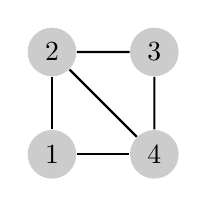
\begin{tikzpicture} [scale=1.3]
      \node[circle,fill=black!20] (v1) at (0,0) {$1$};
      \node[circle,fill=black!20] (v2) at (0,1)  {$2$};
      \node[circle,fill=black!20] (v3) at (1,1) {$3$};
      \node[circle,fill=black!20] (v4) at (1,0) {$4$};
    \draw[thick] (v1) --  (v2) ;
   \draw[thick] (v1) --   (v4);
    \draw[thick] (v2) -- (v3) ;
   \draw[thick] (v2) --    (v4);
  \draw[thick] (v3) --   (v4);
    \end{tikzpicture}
\end{center}

\item \

\begin{center}
    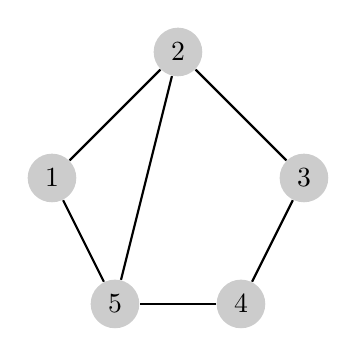
\begin{tikzpicture}[scale=.8]  
      \node[circle,fill=black!20] (v1) at (-1,1) {$1$};
      \node[circle,fill=black!20] (v2) at (1,3)  {$2$};
      \node[circle,fill=black!20] (v3) at (3,1) {$3$};
      \node[circle,fill=black!20] (v4) at (2,-1) {$4$};
     \node[circle,fill=black!20] (v5) at (0,-1) {$5$};
    \draw[thick] (v1) --  (v2) ;
   \draw[thick] (v1) --   (v5);
    \draw[thick] (v2) -- (v3) ;
   \draw[thick] (v2) --    (v5);
  \draw[thick] (v3) --   (v4);
   \draw[thick] (v4) -- (v5);
    \end{tikzpicture}
\end{center}

Do you notice any similarity between the steady states for the graphs?
\end{enumerate}


 \begin{sol}
Write your solution here.
\end{sol}
\clearpage


\item In this problem we will see how calculating powers of (non-Markov) matrices can help understand recurrence relations.  We will use the Fibonacci numbers as an example. The Fibonacci numbers are defined recursively as $F_0 = 0$, $F_1=1$, and for $n \ge 2$, $F_{n} = F_{n-1} + F_{n-2}$.
\begin{enumerate}
\item Let $A = \begin{bmatrix} 1 & 1 \\ 1 & 0 \end{bmatrix}$ and $\vec{u}_0 = (1,0)$.  Note that $\vec{u}_0 = (F_1,F_0)$. Prove that $A^k\vec{u}_0 = (F_{k+1},F_k)$.
\item Verify that the eigenvalues of $A$ are $\lambda_1 = (1 + \sqrt{5})/2$ and $\lambda_2 = (1-\sqrt{5})/2$, with corresponding eigenvectors $\vec{x}_1 = (\lambda_1,1)$ and $\vec{x}_2 = (\lambda_2,1)$.
\item Verify that $\vec{u}_0 = \frac{1}{\lambda_1 - \lambda_2}(\vec{x}_1 - \vec{x}_2)$. [Note you have expressed $\vec{u}_0$ in the basis of eigenvectors.]
\item Write a simple expression for $\vec{u}_k = A^k\vec{u}_0$ in terms of $\vec{x}_1$ and $\vec{x}_2$. [Hint: Use the expression for $\vec{u}_0$ in Part (c).]
\item Since $F_k$ is the second component of $\vec{u}_k$ and the second components of $\vec{x}_1$ and $\vec{x}_2$ are 1, write a simple expression for $F_k$ in terms of $\lambda_1$ and $\lambda_2$.
\item Explain why $F_{100}$ is extremely close to $\frac{1}{\sqrt{5}} \lambda_1^{100}$. (Note that $\lambda_1 - \lambda_2 = \sqrt{5}$), 
\end{enumerate}


 \begin{sol}
Write your solution here.
\end{sol}
\clearpage


\item Let $M$ be an $n \times n$ positive Markov matrix, with $n$ independent eigenvectors $\{\vec{x}_1, \ldots, \vec{x}_n\}$, and $n$ eigenvalues $\{\lambda_1, \lambda_2, \ldots, \lambda_n\}$, where $\lambda_1 = 1$ and $|\lambda_i|<1$ when $i \ge 2$. 
\begin{enumerate}
\item Verify that $\mathbf{1} =(1,1,\ldots,1)$ is in the left nullspace of $M-I$.
\item Verify that $\vec{x}_i$ is in the column space of $M-I$ if $i \ge 2$.
\item Fill in the blank: Since the column space of $(M-I)$ is \hspace{1in}the left nullspace of $(M-I)$, $\vec{x}_i$ is \hspace{1in} $(1,1,\ldots, 1)$ if $i \ge 2$.
\item If $i \ge 2$, explain why the components of $\vec{x}_i$ sum to zero. [Hint: Use Part (c) and the definition of orthogonal.]
\item For any $\vec{v} \in \R^n$, let $\vec{v} = c_1\vec{x}_1 + \cdots + c_n\vec{x}_n$.  Explain why the coefficient $c_1$ is the same for all vectors $\vec{v}$ whose components have a given sum.
\end{enumerate}


 \begin{sol}
Write your solution here.
\end{sol}
\clearpage



\section*{Optional Problems}

\item Prove that if $M$ is a Markov matrix, then the sum of the components of a vector $\vec{v}$ is the same as the sum of the components of $M\vec{v}$.

\item Prove that if $M$ is a positive Markov matrix, the columns of $M^k$ converge to the eigenvector $\vec{x}_1$ with eigenvalue 1, whose components sum to 1.

\item Consider a random walk on the integers from 1 to $n$, where a random walker on $i$ moves to $i+1$ or $i-1$ with equal probability unless they are at 1 or $n$, in which case they move to 2 or $n-1$ with probability 1.  Find the stationary distribution  for various values of $n$.  Can you make a conjecture for the form of the stationary distribution for large values of $n$?

\end{enumerate}




\end{document}